\section{Apparato sperimentale}\label{sec:apparato-sperimentale}
  \subsection{Schema del circuito}\label{subsec:schema-circuito}
  \begin{figure}[h]
    \begin{subfigure}[t]{.47\textwidth}
      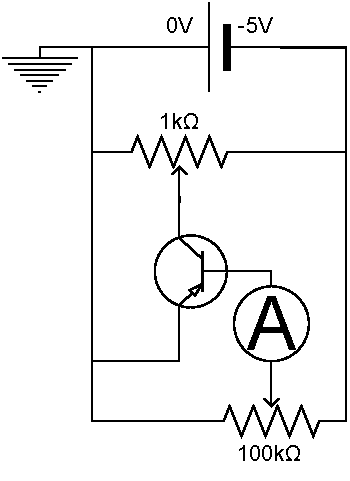
\includegraphics[width=7.75cm]{../assets/circuito-base-current.pdf}
      \caption{
        \emph{
          Schema del circuito usato per selezionare la base current. Il polo positivo del generatore e l'\emph{emitter}
          del transistor sono collegati a terra. I due potenziometri sono collegati ai capi del generatore. L'amperometro
          permette di selezionare $I_b$ agendo sul potenziometro da $100k\Omega$.
        }
      }
      \label{fig:circuito-base-current}
    \end{subfigure}
    %
    \hspace{5mm}
    %
    \begin{subfigure}[t]{.47\textwidth}
      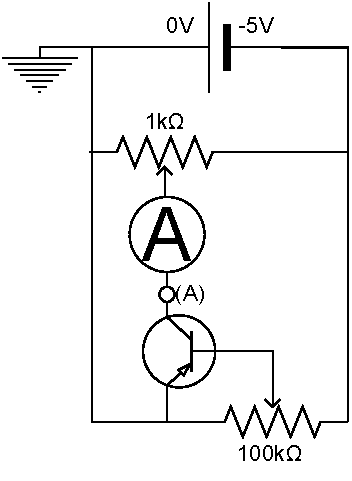
\includegraphics[width=7.75cm]{../assets/circuito.pdf}
      \caption{
        \emph{
          Schema del circuito usato per l'esperimento. Il polo positivo del generatore e l'\emph{emitter}
          del transistor sono collegati a terra. I due potenziometri sono collegati ai capi del generatore. L'oscilloscopio
          è collegato nel punto (A) e misura la tensione tra collettore e terra.
        }
      }
      \label{fig:circuito-prova}
    \end{subfigure}
    \caption{\emph{Schemi circuitali.}}
    \label{fig:circuiti}
  \end{figure}

  Il circuito che abbiamo realizzato è schematizzato in figura \ref{fig:circuiti}, in due configurazioni diverse. In figura \ref{fig:circuito-base-current}
  è riportata la configurazione usata per selezionare la corrente di base $I_b$; in figura \ref{fig:circuito-prova}
  è riportata quella usata durante l'esperimento. Il circuito per l'esperimento è strutturato come segue:
  \begin{enumerate}
    \item%
    Un generatore di tensione è collegato a terra e genera una tensione di $-5V$.
    \item
    Due potenziometri, uno da $1k\Omega$ e uno da $100k\Omega$ sono collegati ai capi del generatore.
    \item
    Un transistor PNP è collegato con la seguente configurazione: $E \to$ terra, $B \to$ potenziometro da $100k\Omega$,
    $C \to$ potenziometro da $1k\Omega$.
    \item
    Un multimetro e un oscilloscopio sono collegati al collettore del transistor, in modo da misurare corrente e tensione
    in uscita.
  \end{enumerate}
  Per selezionare la corrente di base, bisogna realizzare il circuito descritto in figura \ref{fig:circuito-base-current}
  e agire sul potenziometro da $100k\Omega$ fino a che il multimetro non mostra la corrente desiderata.

  \subsection{Materiale e strumenti usati}\label{subsec:materiali}
  Segue una lista del materiale e degli strumenti usati durante la prova:
  \begin{itemize}
    \item%
    Oscilloscopio analogico, modello: \emph{GW Instek GOS-652}.
    \item%
    Multimetro digitale, modello: \emph{ISO-TECH IDM 105}.
    \item%
    Generatore di tensione, modello: \emph{Aim-TTi EB2025T}.
    \item%
    Sonda per oscilloscopio.
    \item%
    Connettori vari (connettori a banana, cavi per la scheda millefori).
    \item%
    Transistor PNP, modello: \emph{2N3906}.
    \item
    Potenziometro da 1k$\Omega$.
    \item
    Potenziometro da 100k$\Omega$.
  \end{itemize}
  Le incertezze degli strumenti utilizzati sono riportate in appendice \ref{sec:incertezze-strumentali}.
  Abbiamo considerato trascurabili le incertezze delle misure fatte con il multimetro, rispetto a quelle fatte con l'oscilloscopio.
